\section{PDE solver}

The graphs \ref{overlap} and \ref{synchro} show the speedup for both of the synchronization methods.

%\begin{figure}[!h]
 % \begin{center}
  %       \resizebox{160mm}{!}{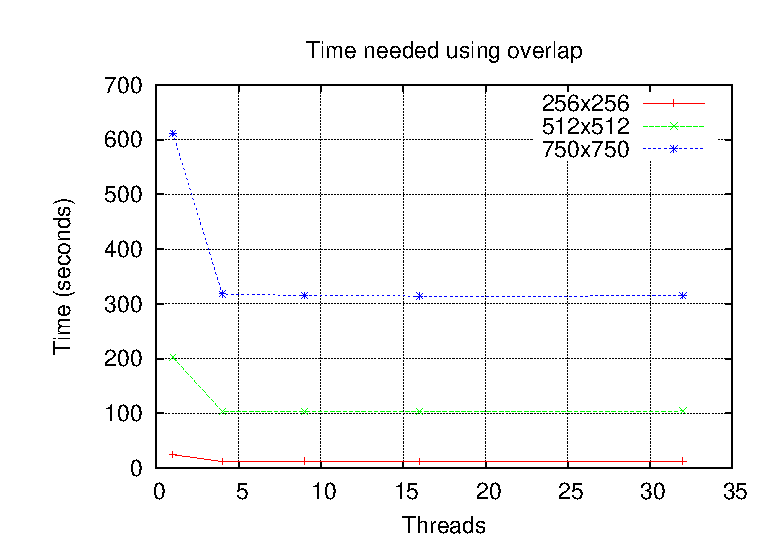
\includegraphics{pic/graph_over_time.eps}}
  %\end{center}
  %\caption{Time needed using overlap}
%\end{figure}

\begin{figure}[H]
  \begin{center}
         \resizebox{160mm}{!}{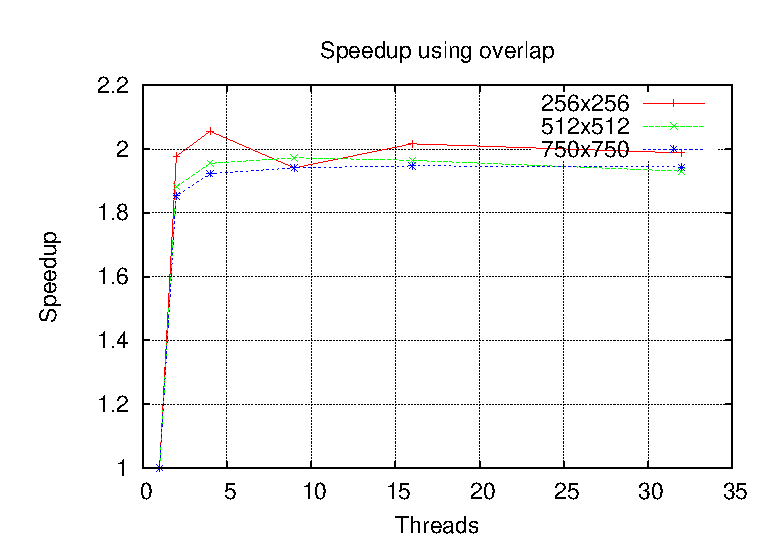
\includegraphics{pic/graph_over.eps}}
  \end{center}
  \caption{Speedup using overlap}
  \label{overlap}
\end{figure}

%\begin{figure}[!h]
 % \begin{center}
  %       \resizebox{160mm}{!}{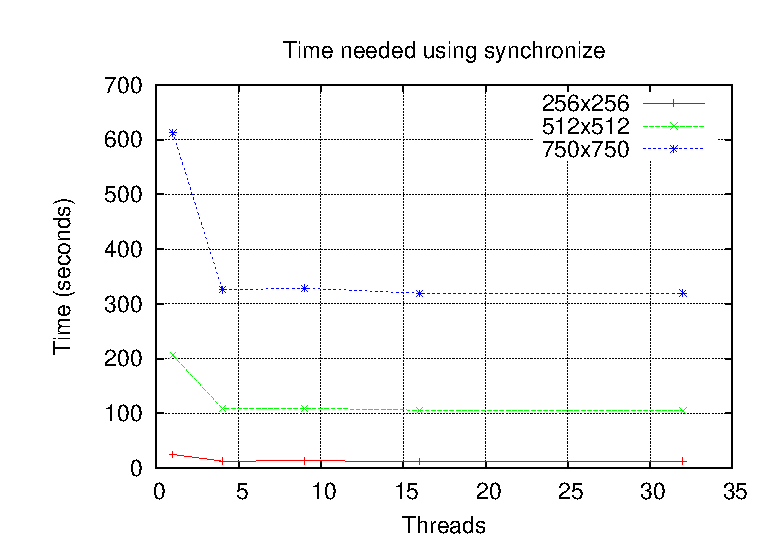
\includegraphics{pic/graph_synchro_time.eps}}
 % \end{center}
 % \caption{Time needed using synchronize}
%\end{figure}

\begin{figure}[!h]
  \begin{center}
         \resizebox{160mm}{!}{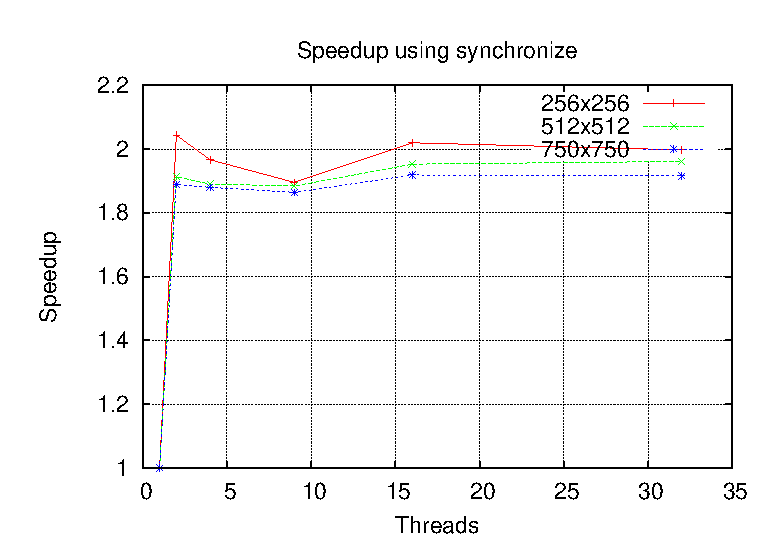
\includegraphics{pic/graph_synchro.eps}}
  \end{center}
  \caption{Speedup using synchronize}
  \label{synchro}
\end{figure}

As we can see in those pictures, the speedup remains the same for both of the methods. The speedup is only good during the first step, that is from 1 to 4 threads, and remains more or less the same because of the synchronization. Indeed, regardless of the method we choose, threads must be synchronized.

When several threads are used (from 2 to 32 in our example), the execution time does not change much. The only change that is worth notifying is the one that occurs when we go from 1 thread to 2 threads. At that time, the execution is basically divided by two. However, this cannot be said for the rest of the graph. This is because of synchronization. Indeed, using several threads increases performances but brings also the need to synchronize them. The time spent for this hinders the performances and creates some kind of lower bound the execution time cannot (around half of the time on one thread).
